\documentclass[11pt, a4paper]{article}
\usepackage{pdfpages}
\usepackage{parallel}
\usepackage[T2A]{fontenc}
\usepackage{ucs}
\usepackage[utf8x]{inputenc}
\usepackage[polish,english,russian]{babel}
\usepackage{hyperref}
\usepackage{rotating}
\usepackage[inner=2cm,top=1.8cm,outer=2cm,bottom=2.3cm,nohead]{geometry}
\usepackage{listings}
\usepackage{graphicx}
\usepackage{wrapfig}
\usepackage{longtable}
\usepackage{indentfirst}
\usepackage{array}
\usepackage{tikzsymbols}
\usepackage{soul}
\usepackage[ruled,vlined]{algorithm2e}
%\counterwithout{figure}{section} 

\usepackage{url}
\makeatletter
\g@addto@macro{\UrlBreaks}{\UrlOrds}
\makeatother

\newcolumntype{P}[1]{>{\raggedright\arraybackslash}p{#1}}
\frenchspacing
\usepackage{fixltx2e} %text sub- and superscripts
\usepackage{icomma} % коскі ў матэматычным рэжыме
\PreloadUnicodePage{4}

\newcommand{\longpage}{\enlargethispage{\baselineskip}}
\newcommand{\shortpage}{\enlargethispage{-\baselineskip}}

\def\switchlang#1{\expandafter\csname switchlang#1\endcsname}
\def\switchlangbe{
\let\saverefname=\refname%
\def\refname{Літаратура}%
\def\figurename{Іл.}%
}
\def\switchlangen{
\let\saverefname=\refname%
\def\refname{References}%
\def\figurename{Fig.}%
}
\def\switchlangru{
\let\saverefname=\refname%
\let\savefigurename=\figurename%
\def\refname{Литература}%
\def\figurename{Рис.}%
}

\hyphenation{admi-ni-stra-tive}
\hyphenation{ex-pe-ri-ence}
\hyphenation{fle-xi-bi-li-ty}
\hyphenation{Py-thon}
\hyphenation{ma-the-ma-ti-cal}
\hyphenation{re-ported}
\hyphenation{imp-le-menta-tions}
\hyphenation{pro-vides}
\hyphenation{en-gi-neering}
\hyphenation{com-pa-ti-bi-li-ty}
\hyphenation{im-pos-sible}
\hyphenation{desk-top}
\hyphenation{elec-tro-nic}
\hyphenation{com-pa-ny}
\hyphenation{de-ve-lop-ment}
\hyphenation{de-ve-loping}
\hyphenation{de-ve-lop}
\hyphenation{da-ta-ba-se}
\hyphenation{plat-forms}
\hyphenation{or-ga-ni-za-tion}
\hyphenation{pro-gramming}
\hyphenation{in-stru-ments}
\hyphenation{Li-nux}
\hyphenation{sour-ce}
\hyphenation{en-vi-ron-ment}
\hyphenation{Te-le-pathy}
\hyphenation{Li-nux-ov-ka}
\hyphenation{Open-BSD}
\hyphenation{Free-BSD}
\hyphenation{men-ti-on-ed}
\hyphenation{app-li-ca-tion}

\def\progref!#1!{\texttt{#1}}
\renewcommand{\arraystretch}{2} %Іначай формулы ў матрыцы зліпаюцца з лініямі
\usepackage{array}

\def\interview #1 (#2), #3, #4, #5\par{

\section[#1, #3, #4]{#1 -- #3, #4}
\def\qname{LVEE}
\def\aname{#1}
\def\q ##1\par{{\noindent \bf \qname: ##1 }\par}
\def\a{{\noindent \bf \aname: } \def\qname{L}\def\aname{#2}}
}

\def\interview* #1 (#2), #3, #4, #5\par{

\section*{#1\\{\small\rm #3, #4. #5}}
\ifx\ParallelWhichBox\undefined%
    \addcontentsline{toc}{section}{#1, #3, #4}%
\else%
\ifnum\ParallelWhichBox=0%
    \addcontentsline{toc}{section}{#1, #3, #4}%
\fi\fi%

\def\qname{LVEE}
\def\aname{#1}
\def\q ##1\par{{\noindent \bf \qname: ##1 }\par}
\def\a{{\noindent \bf \aname: } \def\qname{L}\def\aname{#2}}
}

\newcommand{\interviewfooter}[1]{
\vskip 1em
\noindent \textit{#1}
}

\switchlang{en}
\begin{document}

\title{1986 "--- Honeywell microLYNX trackball}
\date{}
\maketitle
\selectlanguage{english}
The microLYNX trackball (or “$\mu LYNX$” if Greek characters are allowed) shown in figure \ref{fig:microLYNXPic} was manufactured in California by Honeywell, a subsidiary of Disc Instruments. Having appeared in 1986 or a year earlier (some of the advertising materials are dated 1985), the trackball proved to be a long-liver and subsequently withstood many incarnations as the model “LX200”, which differed in connection interfaces, electronics and were often rebranded under different company names \cite{lx200}.

\begin{figure}[h]
    \centering
    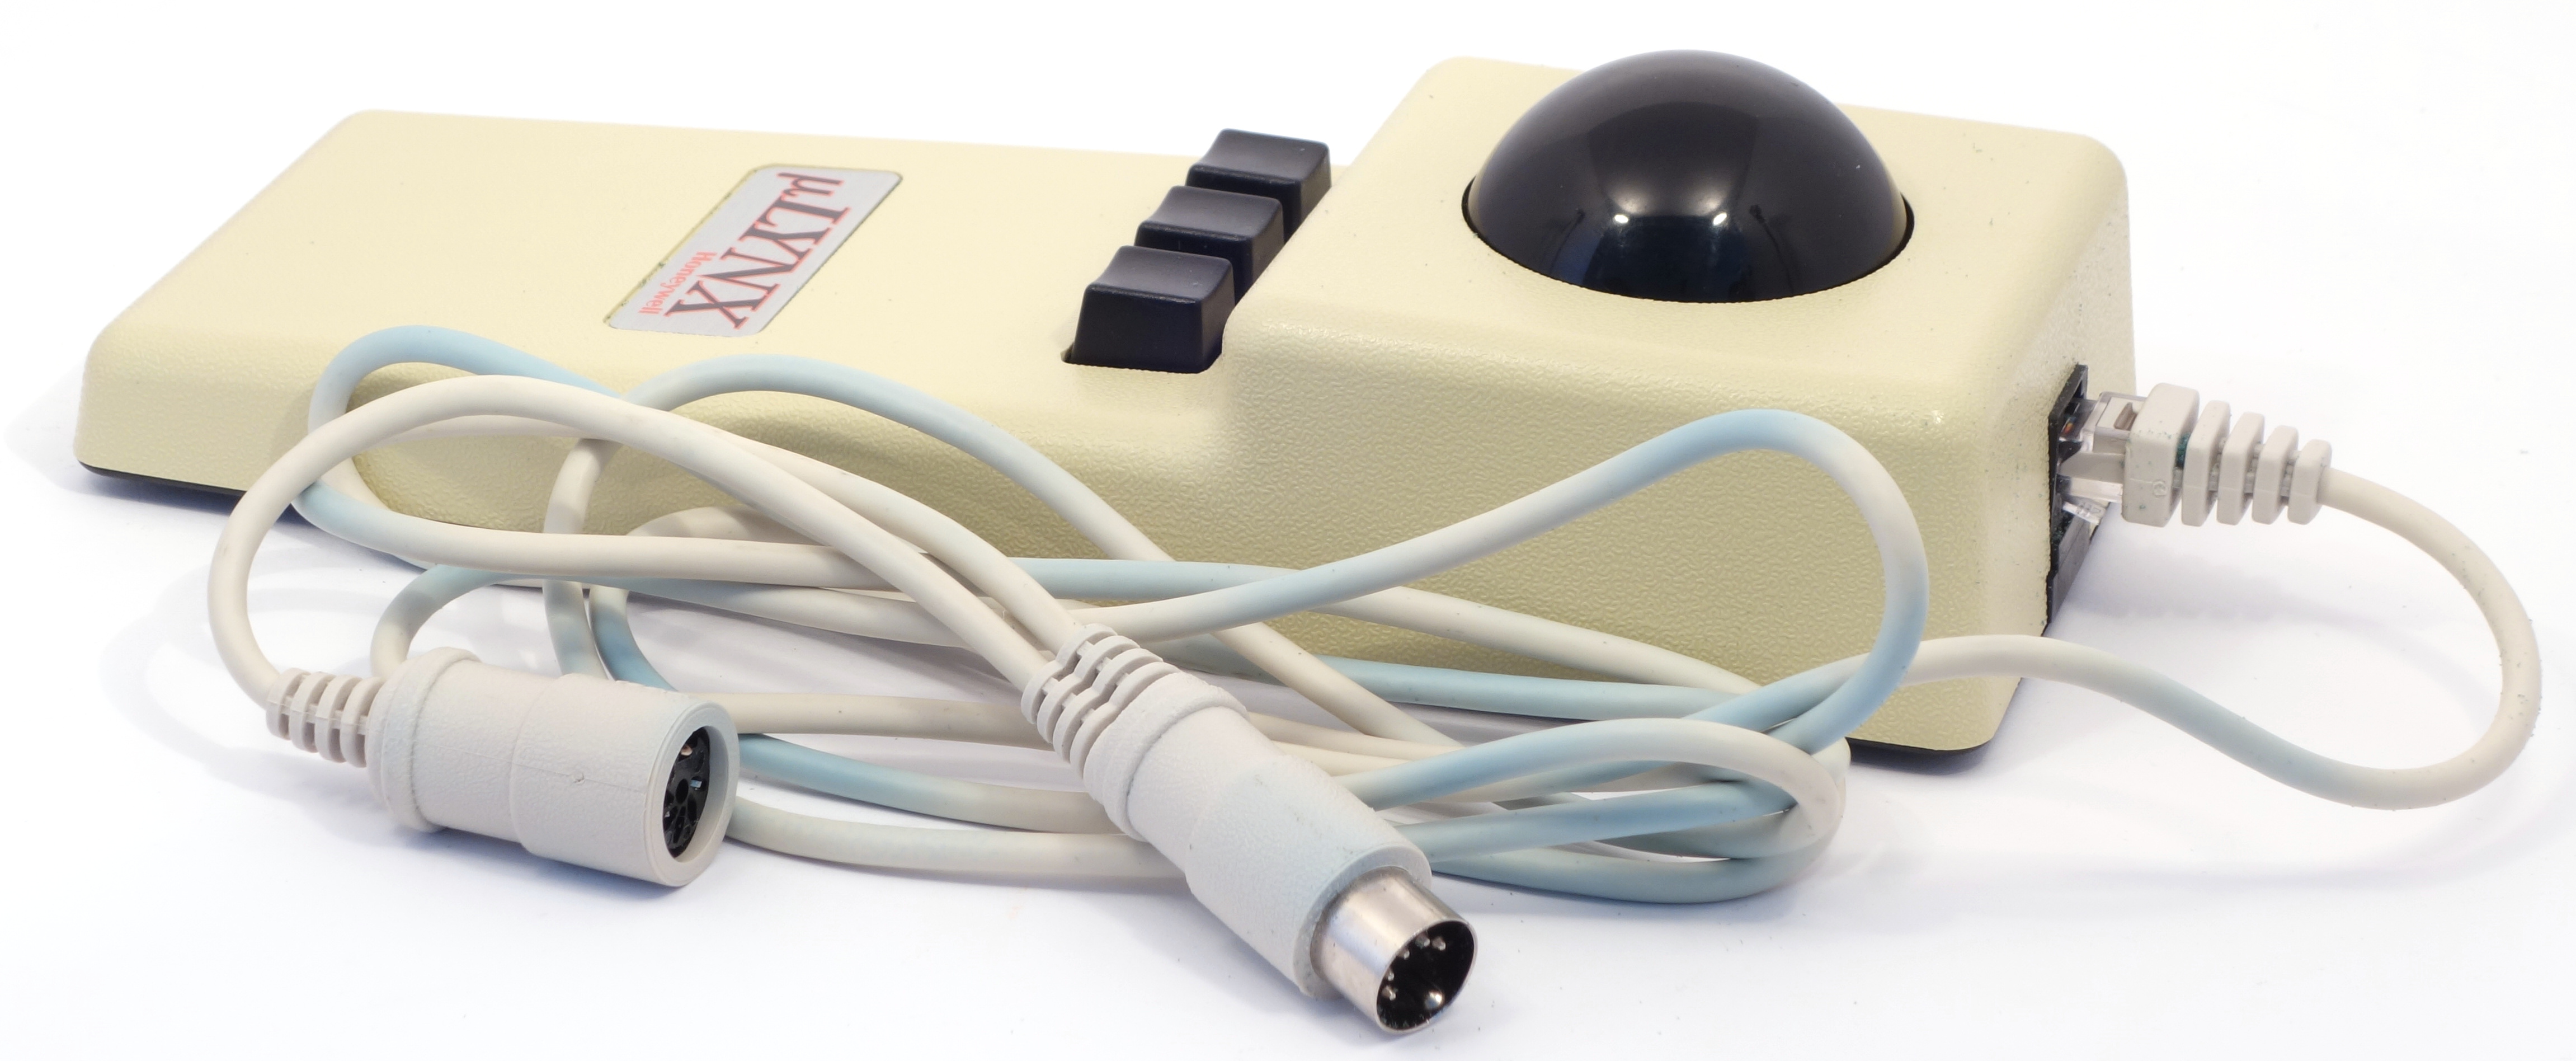
\includegraphics[scale=0.45]{1986_honeywell_microlynx_trackball/pic_30.jpg}
    \caption{Honeywell microLYNX trackball}
    \label{fig:microLYNXPic}
\end{figure}

As you can see, the device is made in a minimalist design, equipped with a large black ball recessed in a beige body with an extended wrist rest \ref{fig:microLYNXTopBottom}. The ball fits snugly to the edges of the hole in the device case, which protects well from debris getting inside the trackball, but makes it impossible to remove the ball for cleaning without disassembling the case. In front of the ball are three buttons with keycaps identical to the keys of the classic full-size keyboard of that time.

\begin{figure}[h]
    \centering
    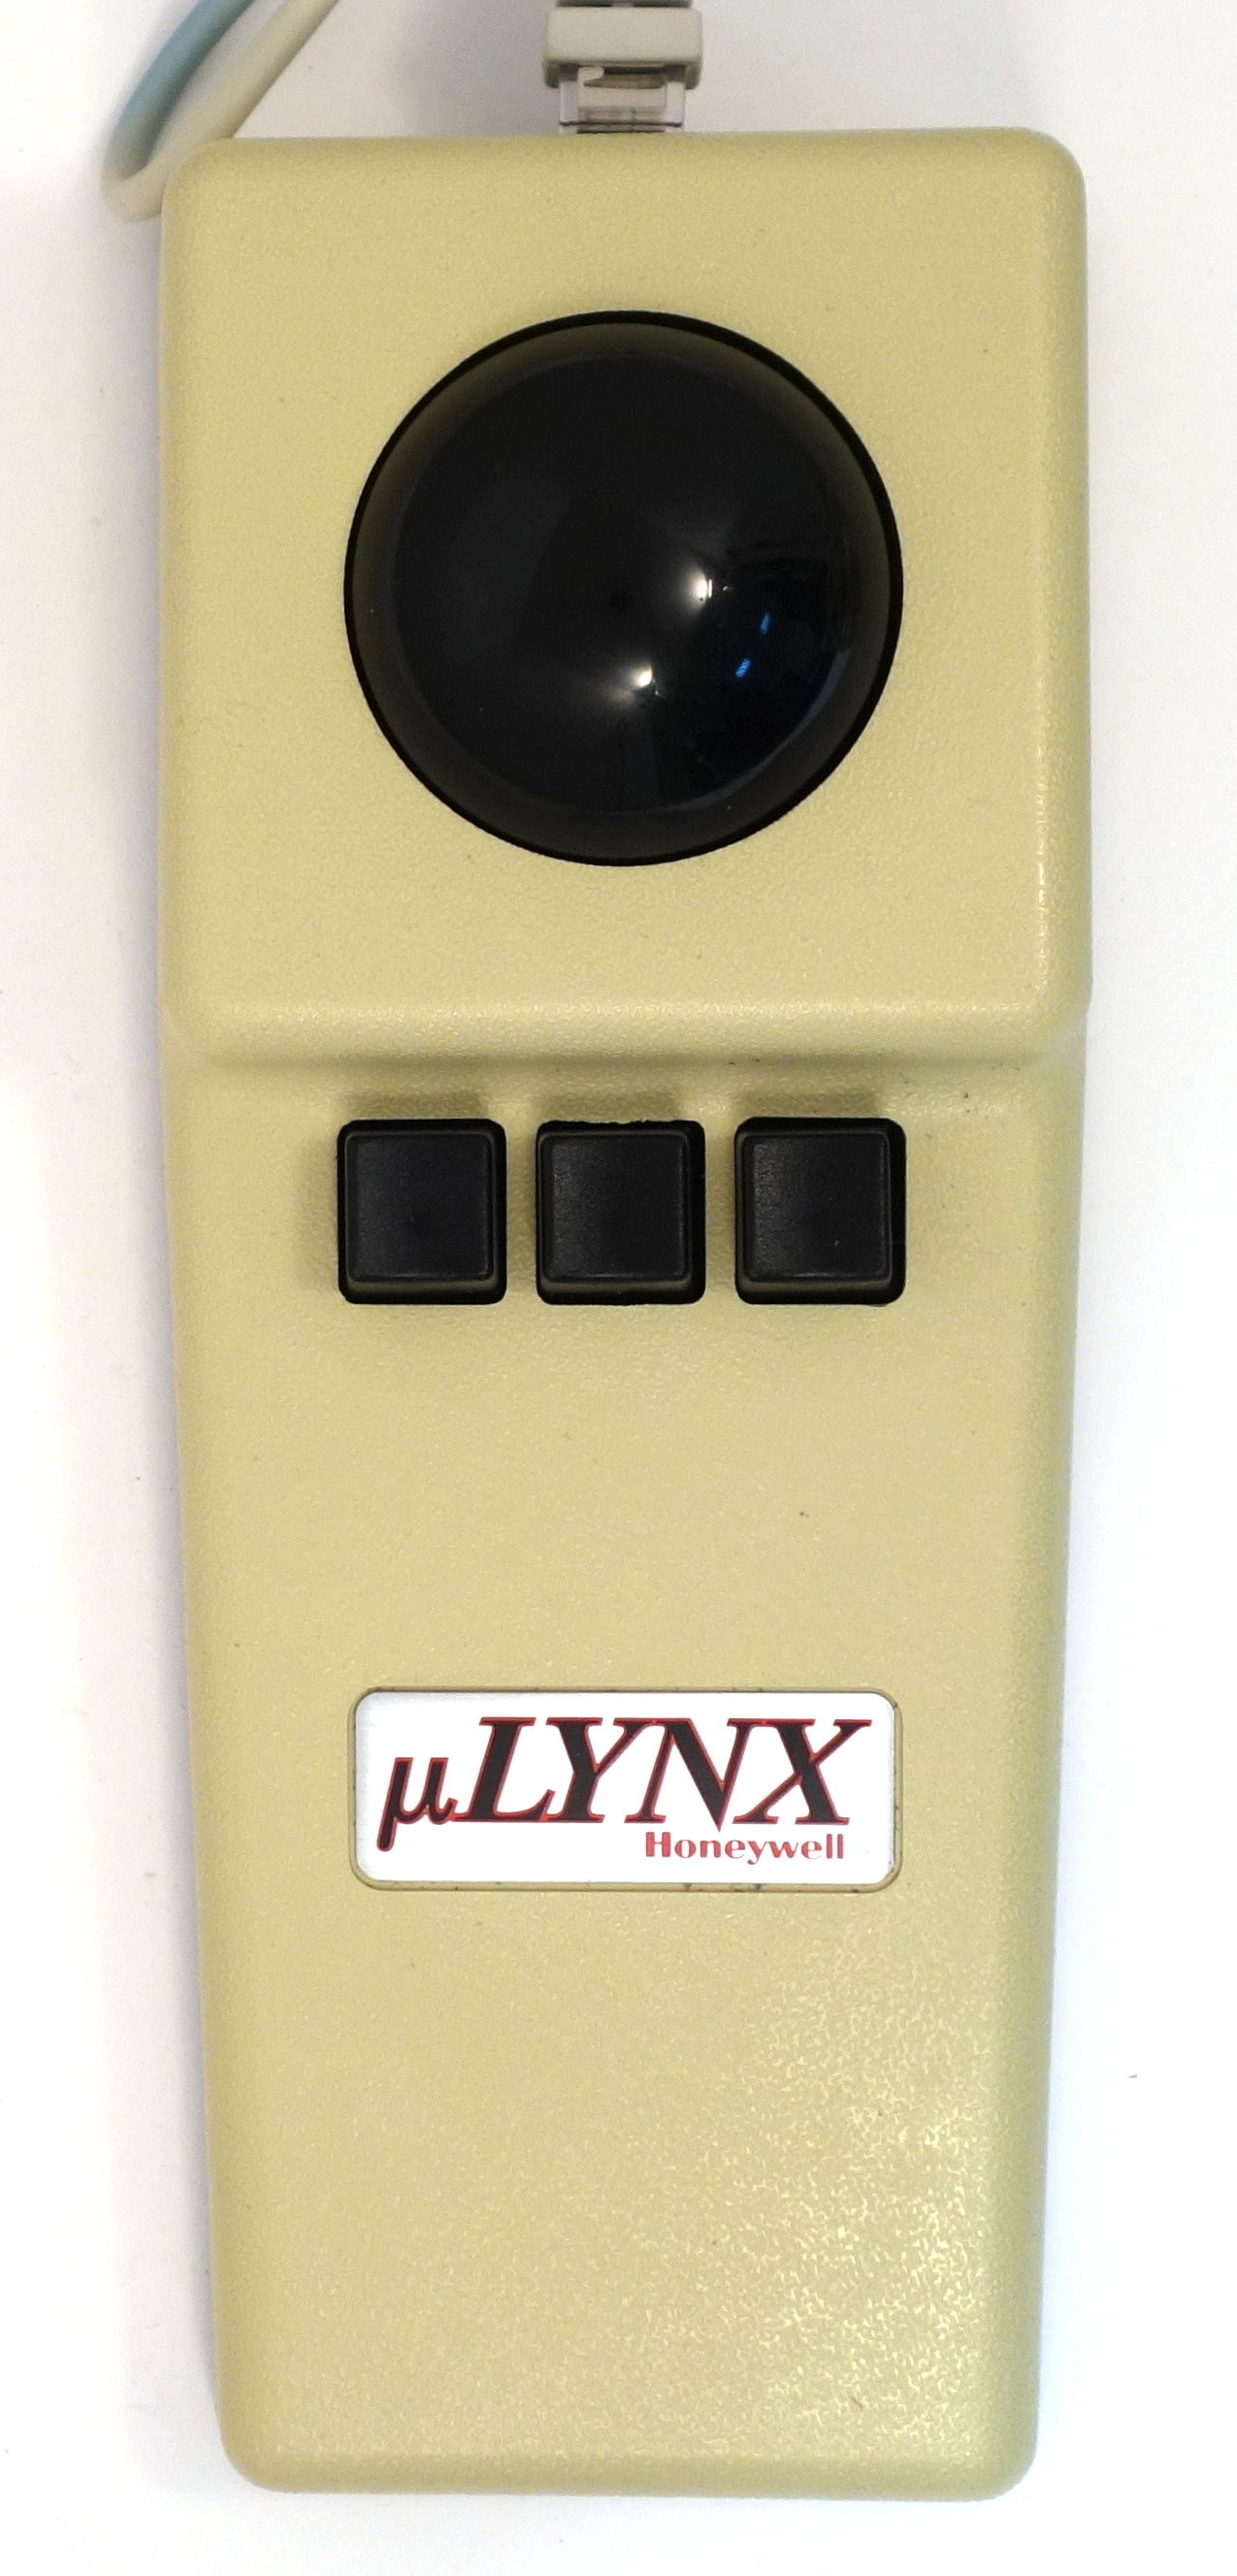
\includegraphics[scale=0.4]{1986_honeywell_microlynx_trackball/top_30.jpg}
    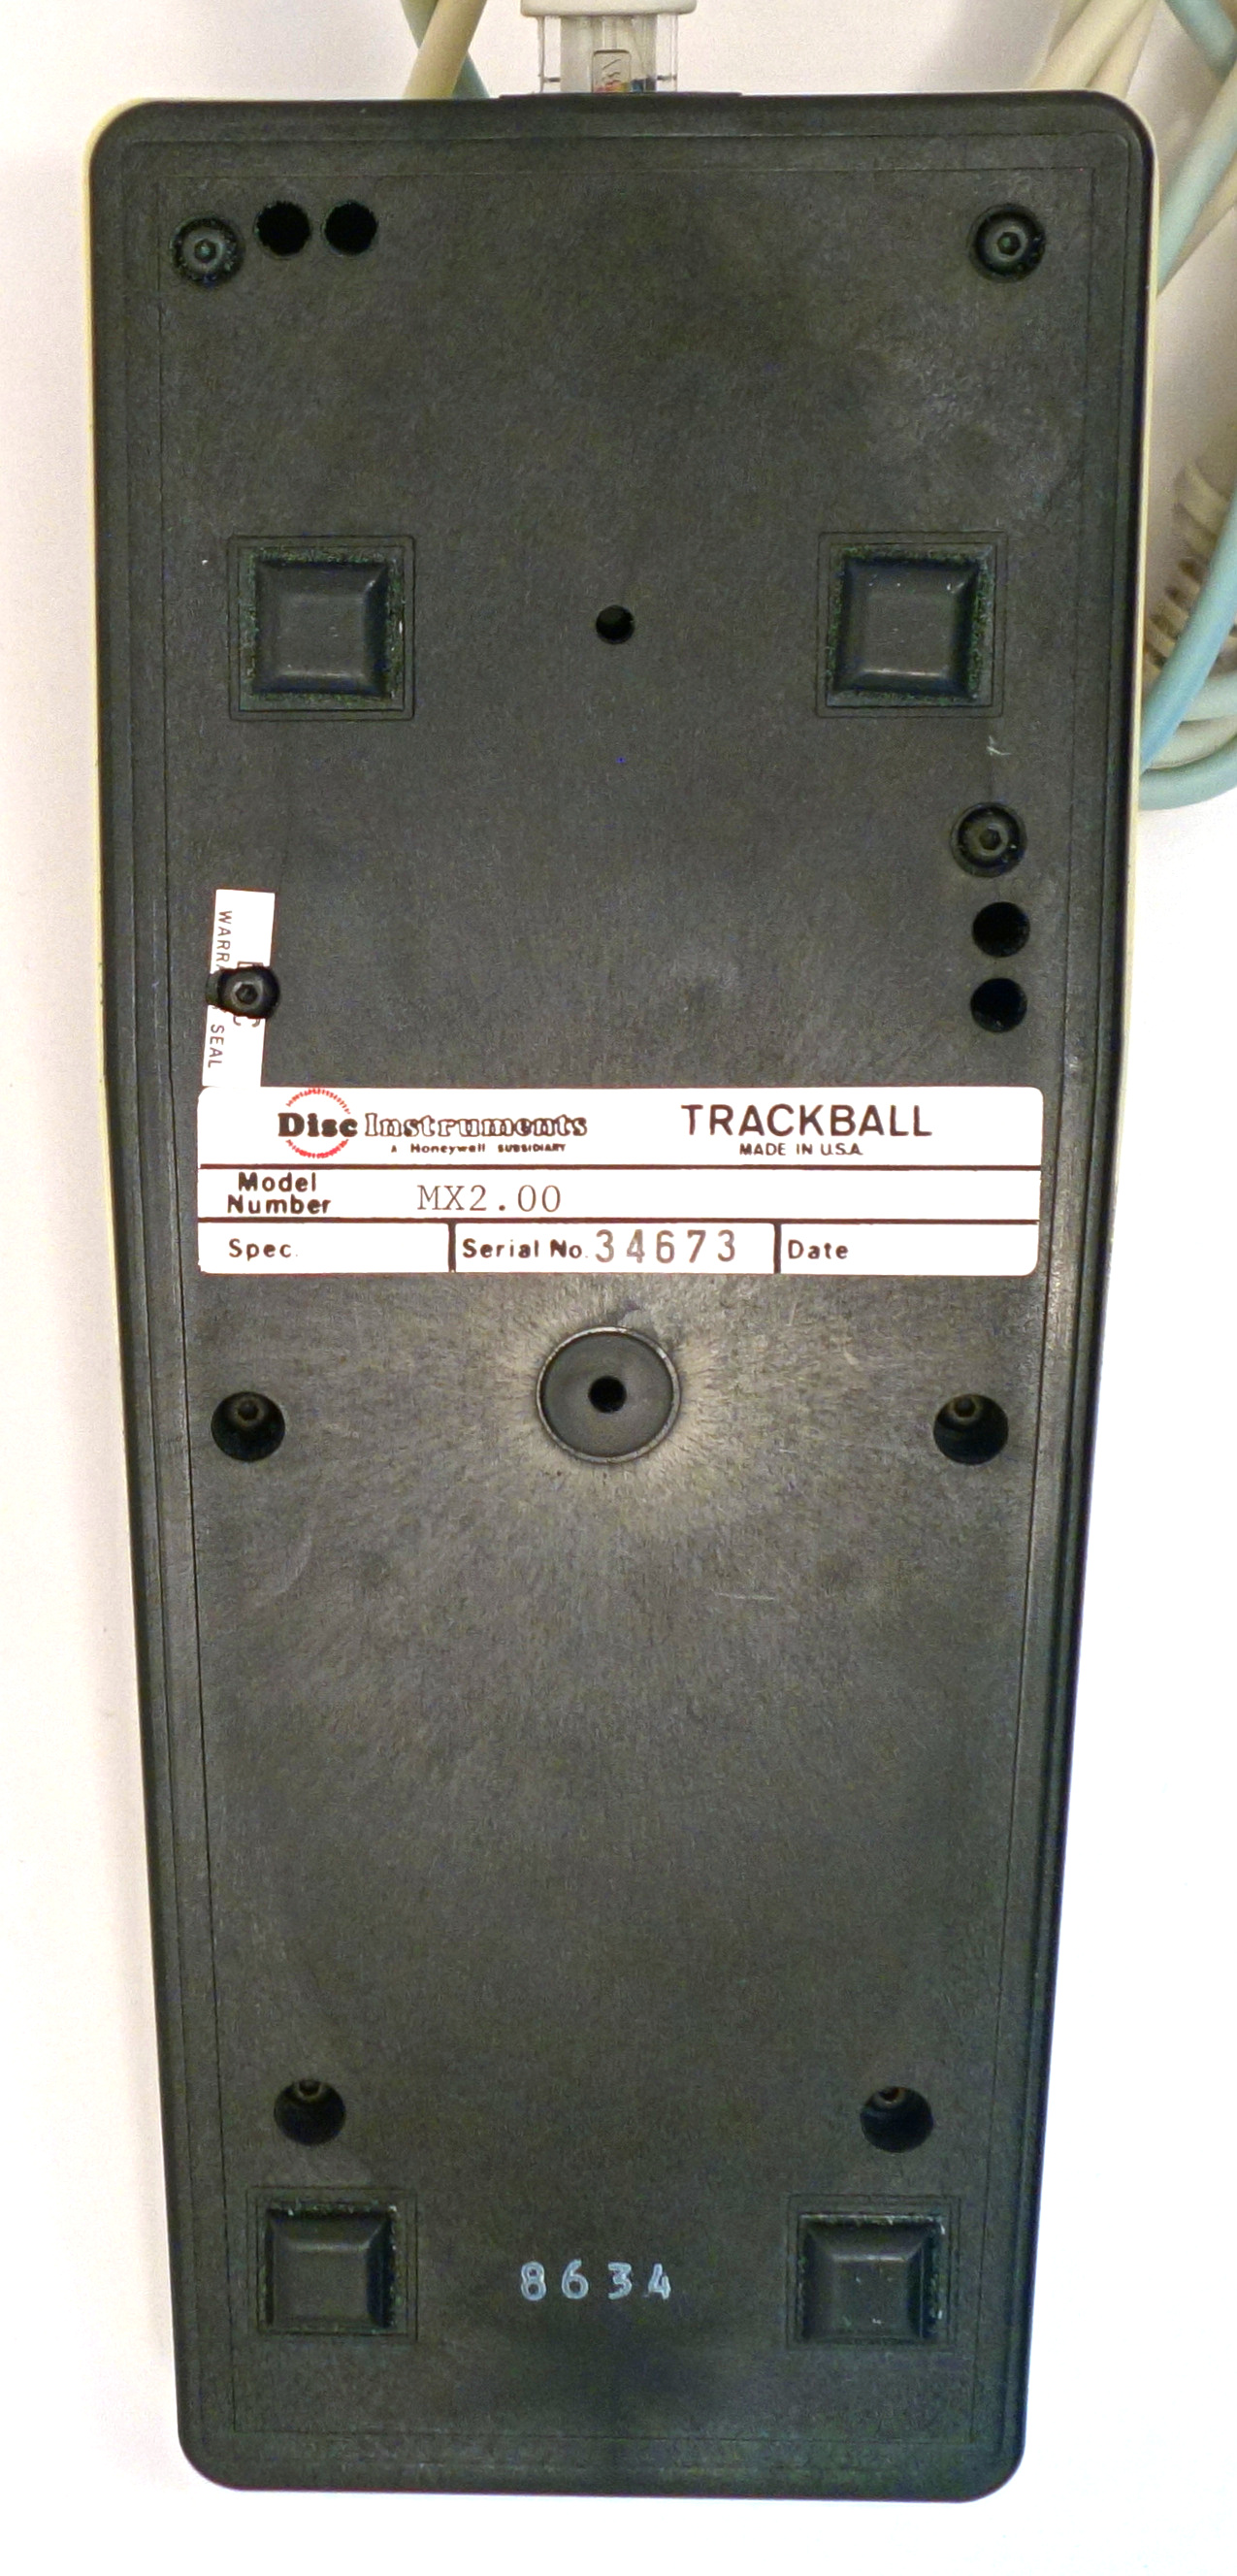
\includegraphics[scale=0.4]{1986_honeywell_microlynx_trackball/bottom_30.jpg}
    \caption{microLYNX, top and bottom views}
    \label{fig:microLYNXTopBottom}
\end{figure}

Apparently, there were two early versions of the “LX200”: the comLYNX model had a serial \cite{comlynx} interface, the quadLYNX version was the most electronically simple quadrature device connected to the bus interface, while the most unusual of the three options, microLYNX, used the keyboard port as a connection interface, actually being included in the break of the keyboard cable. Later, variants with PS/2 interface also appeared.

By default, microLYNX operates in “text mode”, and turning the ball has the same effect as pressing the cursor keys on the keyboard: in fact, when the ball moves, the trackball generates and sends scan codes of the cursor keys to the computer. Trackball buttons are programmable: the user can configure the button to issue from 1 to 30 key codes in the form of macros. You can also adjust the cursor movement speed (how often the cursor key codes are generated).

The microLYNX driver can emulate a Microsoft mouse for graphics programs under DOS, and the user can use the trackball to move the cursor and do dragging to select text or move graphics (the two external buttons in front of the ball can be used to drag).

\begin{figure}[h]
    \centering
    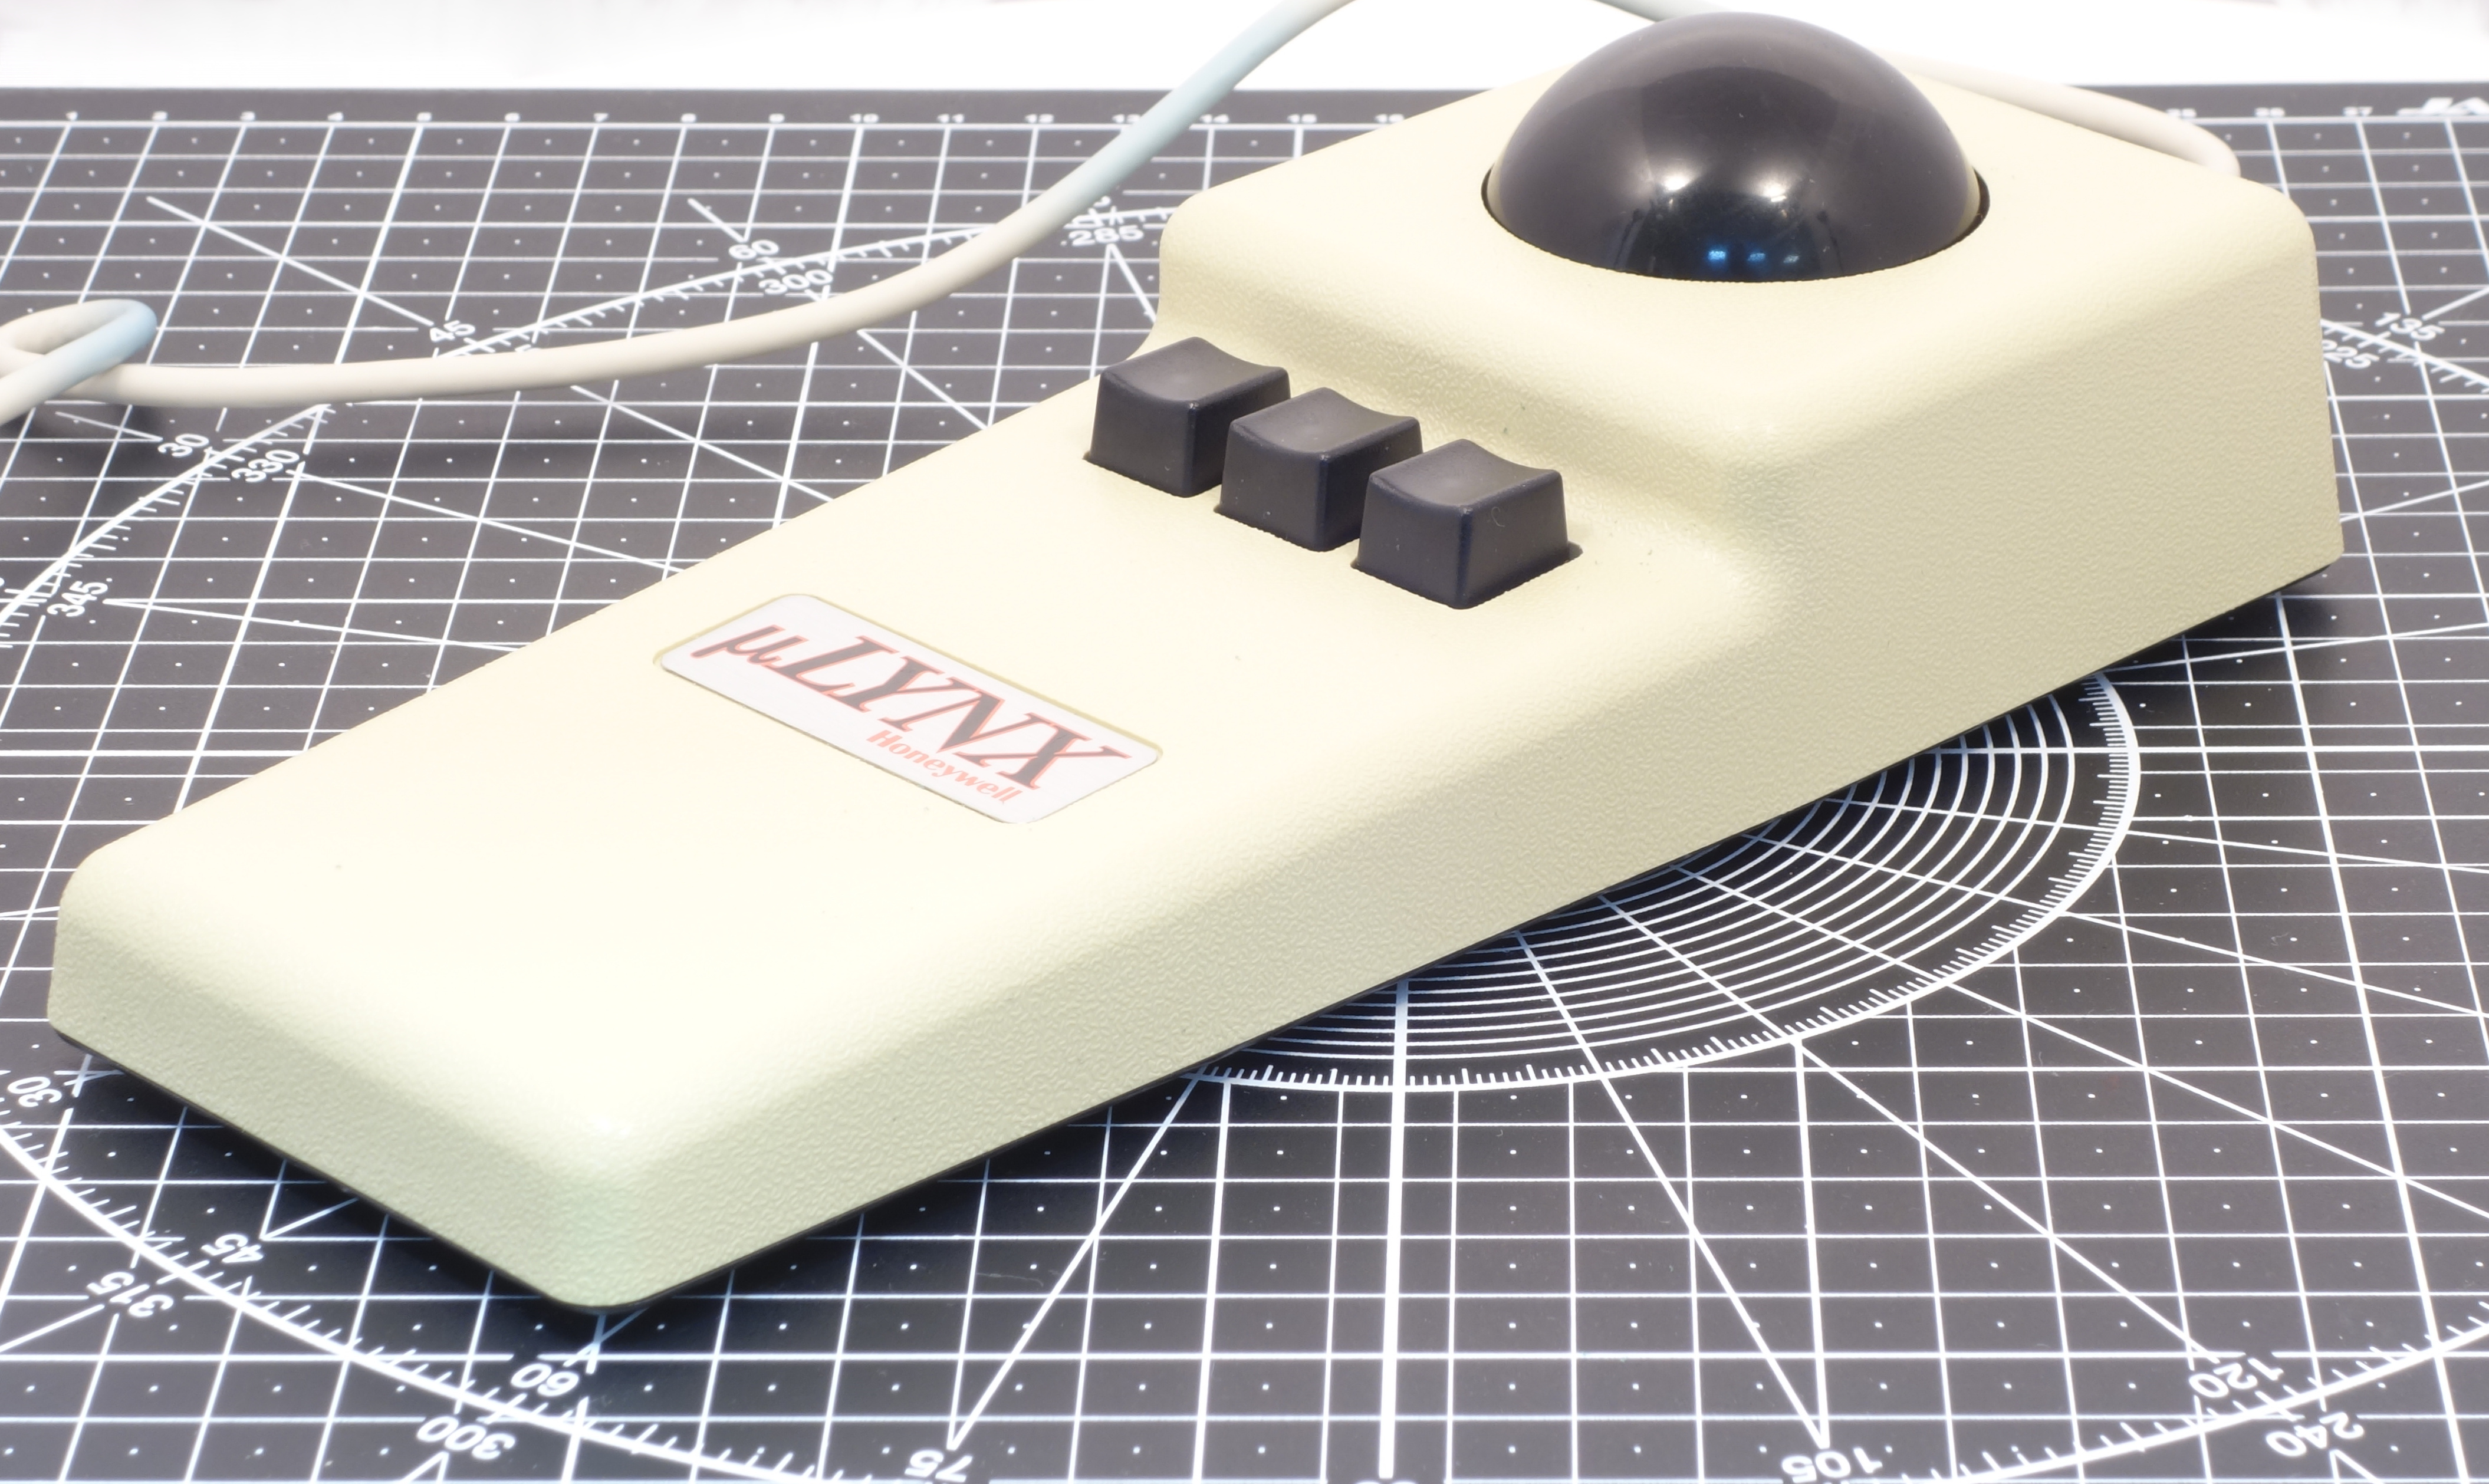
\includegraphics[scale=0.4]{1986_honeywell_microlynx_trackball/size.jpg}
    \caption{microLYNX on a graduated pad with a grid step of 1~cm}
    \label{fig:microLYNXSize}
\end{figure}

However, given the size of the device (figure \ref{fig:microLYNXSize}), holding down the button while the ball is moving is a tricky maneuver at best. Honeywell solved this problem with the comLYNX trackball, which can use the middle button as a \cite{comlynx} drag latch. First, the middle button is pressed, then the left or right button, and this programmatically fixes the selected button in the pressed position. Repeated pressing of any of the three buttons disables this mode. However, microLYNX does not support this feature.

The trackball comes with two sets of software: a DOS driver that emulates a Microsoft mouse, and a separate DOS resident program that shows a pop-up menu and also allows you to program keyboard macros for the trackball buttons and cursor movement.

In addition, configuration can be performed without using a driver, in “alternative mode”, which is activated by pressing the “Ctrl + Alt + Shift” combination on the computer keyboard (due to the nature of the connection, microLYNX “listens” to everything that the keyboard sends to the computer). When entering this mode, the trackball prints text prompts to standard output (as if the user had just typed them) and asks the user to type special commands on the keyboard that change its settings.

\begin{figure}[h]
    \centering
    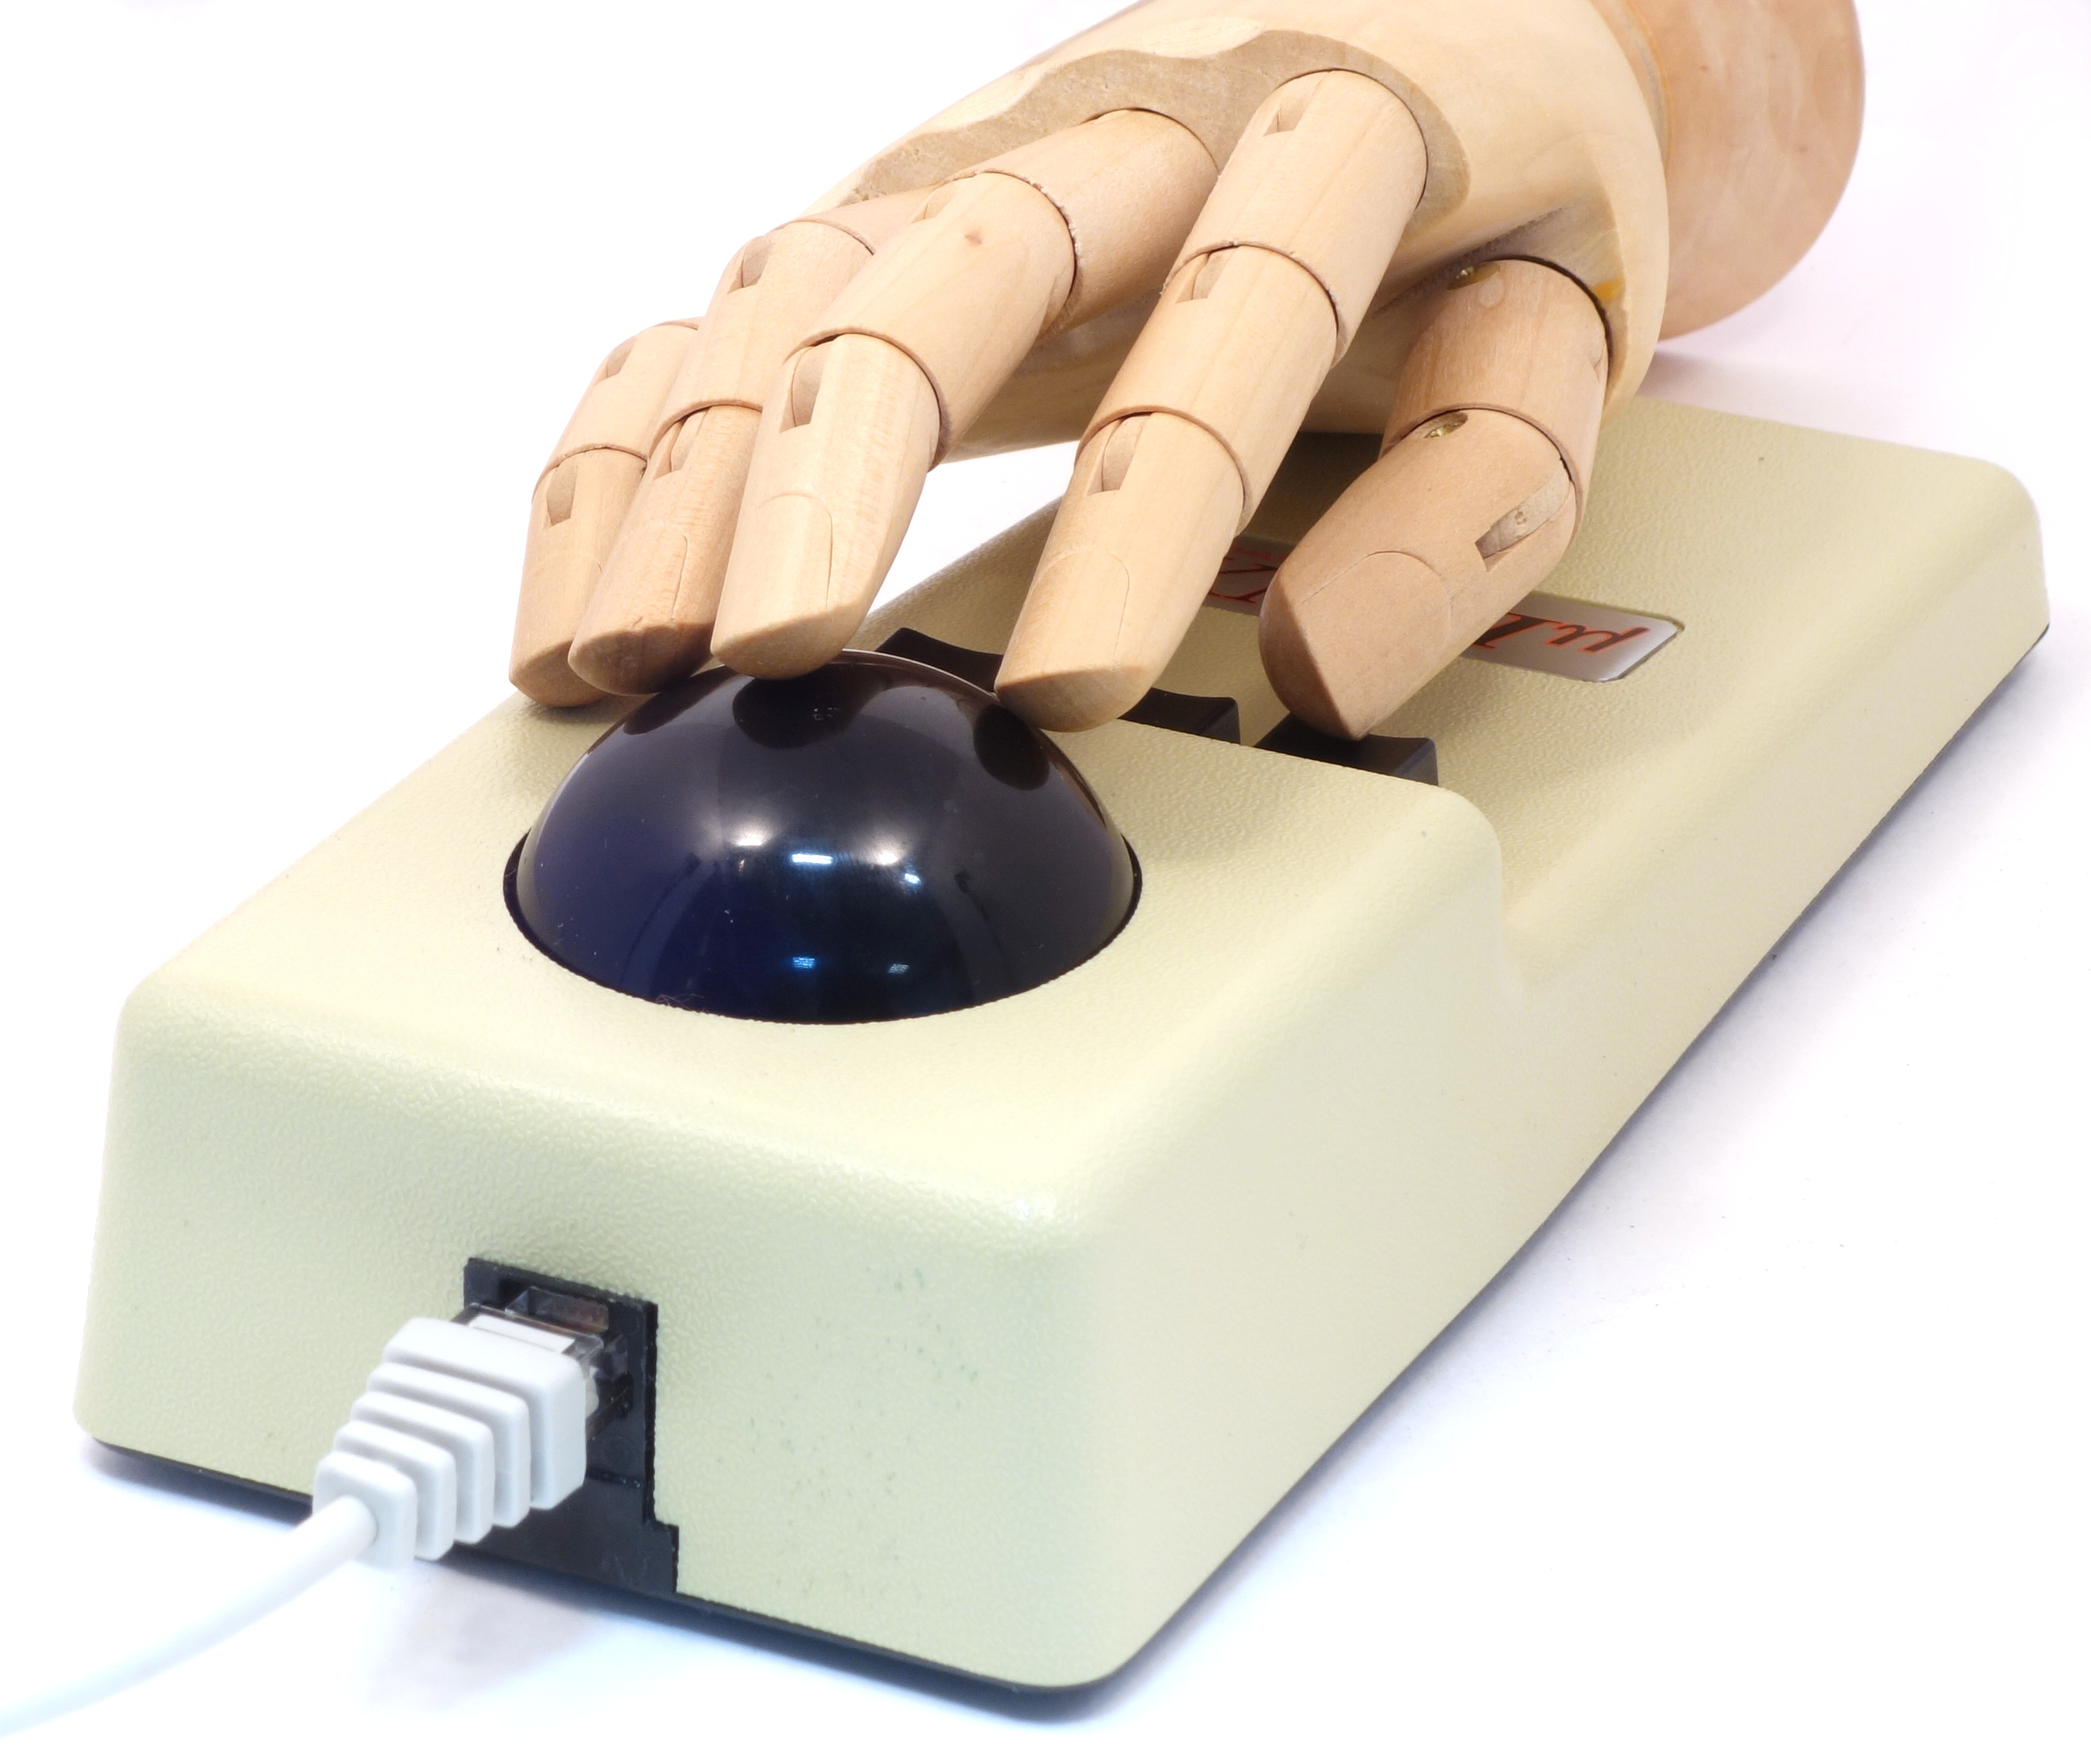
\includegraphics[scale=0.4]{1986_honeywell_microlynx_trackball/hand_60.jpg}
    \caption{microLYNX with a human hand model}
    \label{fig:microLYNXHand}
\end{figure}

In terms of ergonomics, the size of the trackball, the wrist rest, and the rounded edges and corners create a fairly comfortable working environment (figure \ref{fig:microLYNXHand}). However, the buttons are located far from the ball and significantly lower in height, which deprives the user of both the ability to press them with one hand without moving the hand, and with two hands, since the buttons are covered by the palm of the hand when the user rotates the ball. Therefore, microLYNX is difficult to use in a graphical interface that requires intensive work with both frequent cursor movements and button presses. However, the trackball can be quite effective in various industrial applications.

\begin{figure}[h]
    \centering
    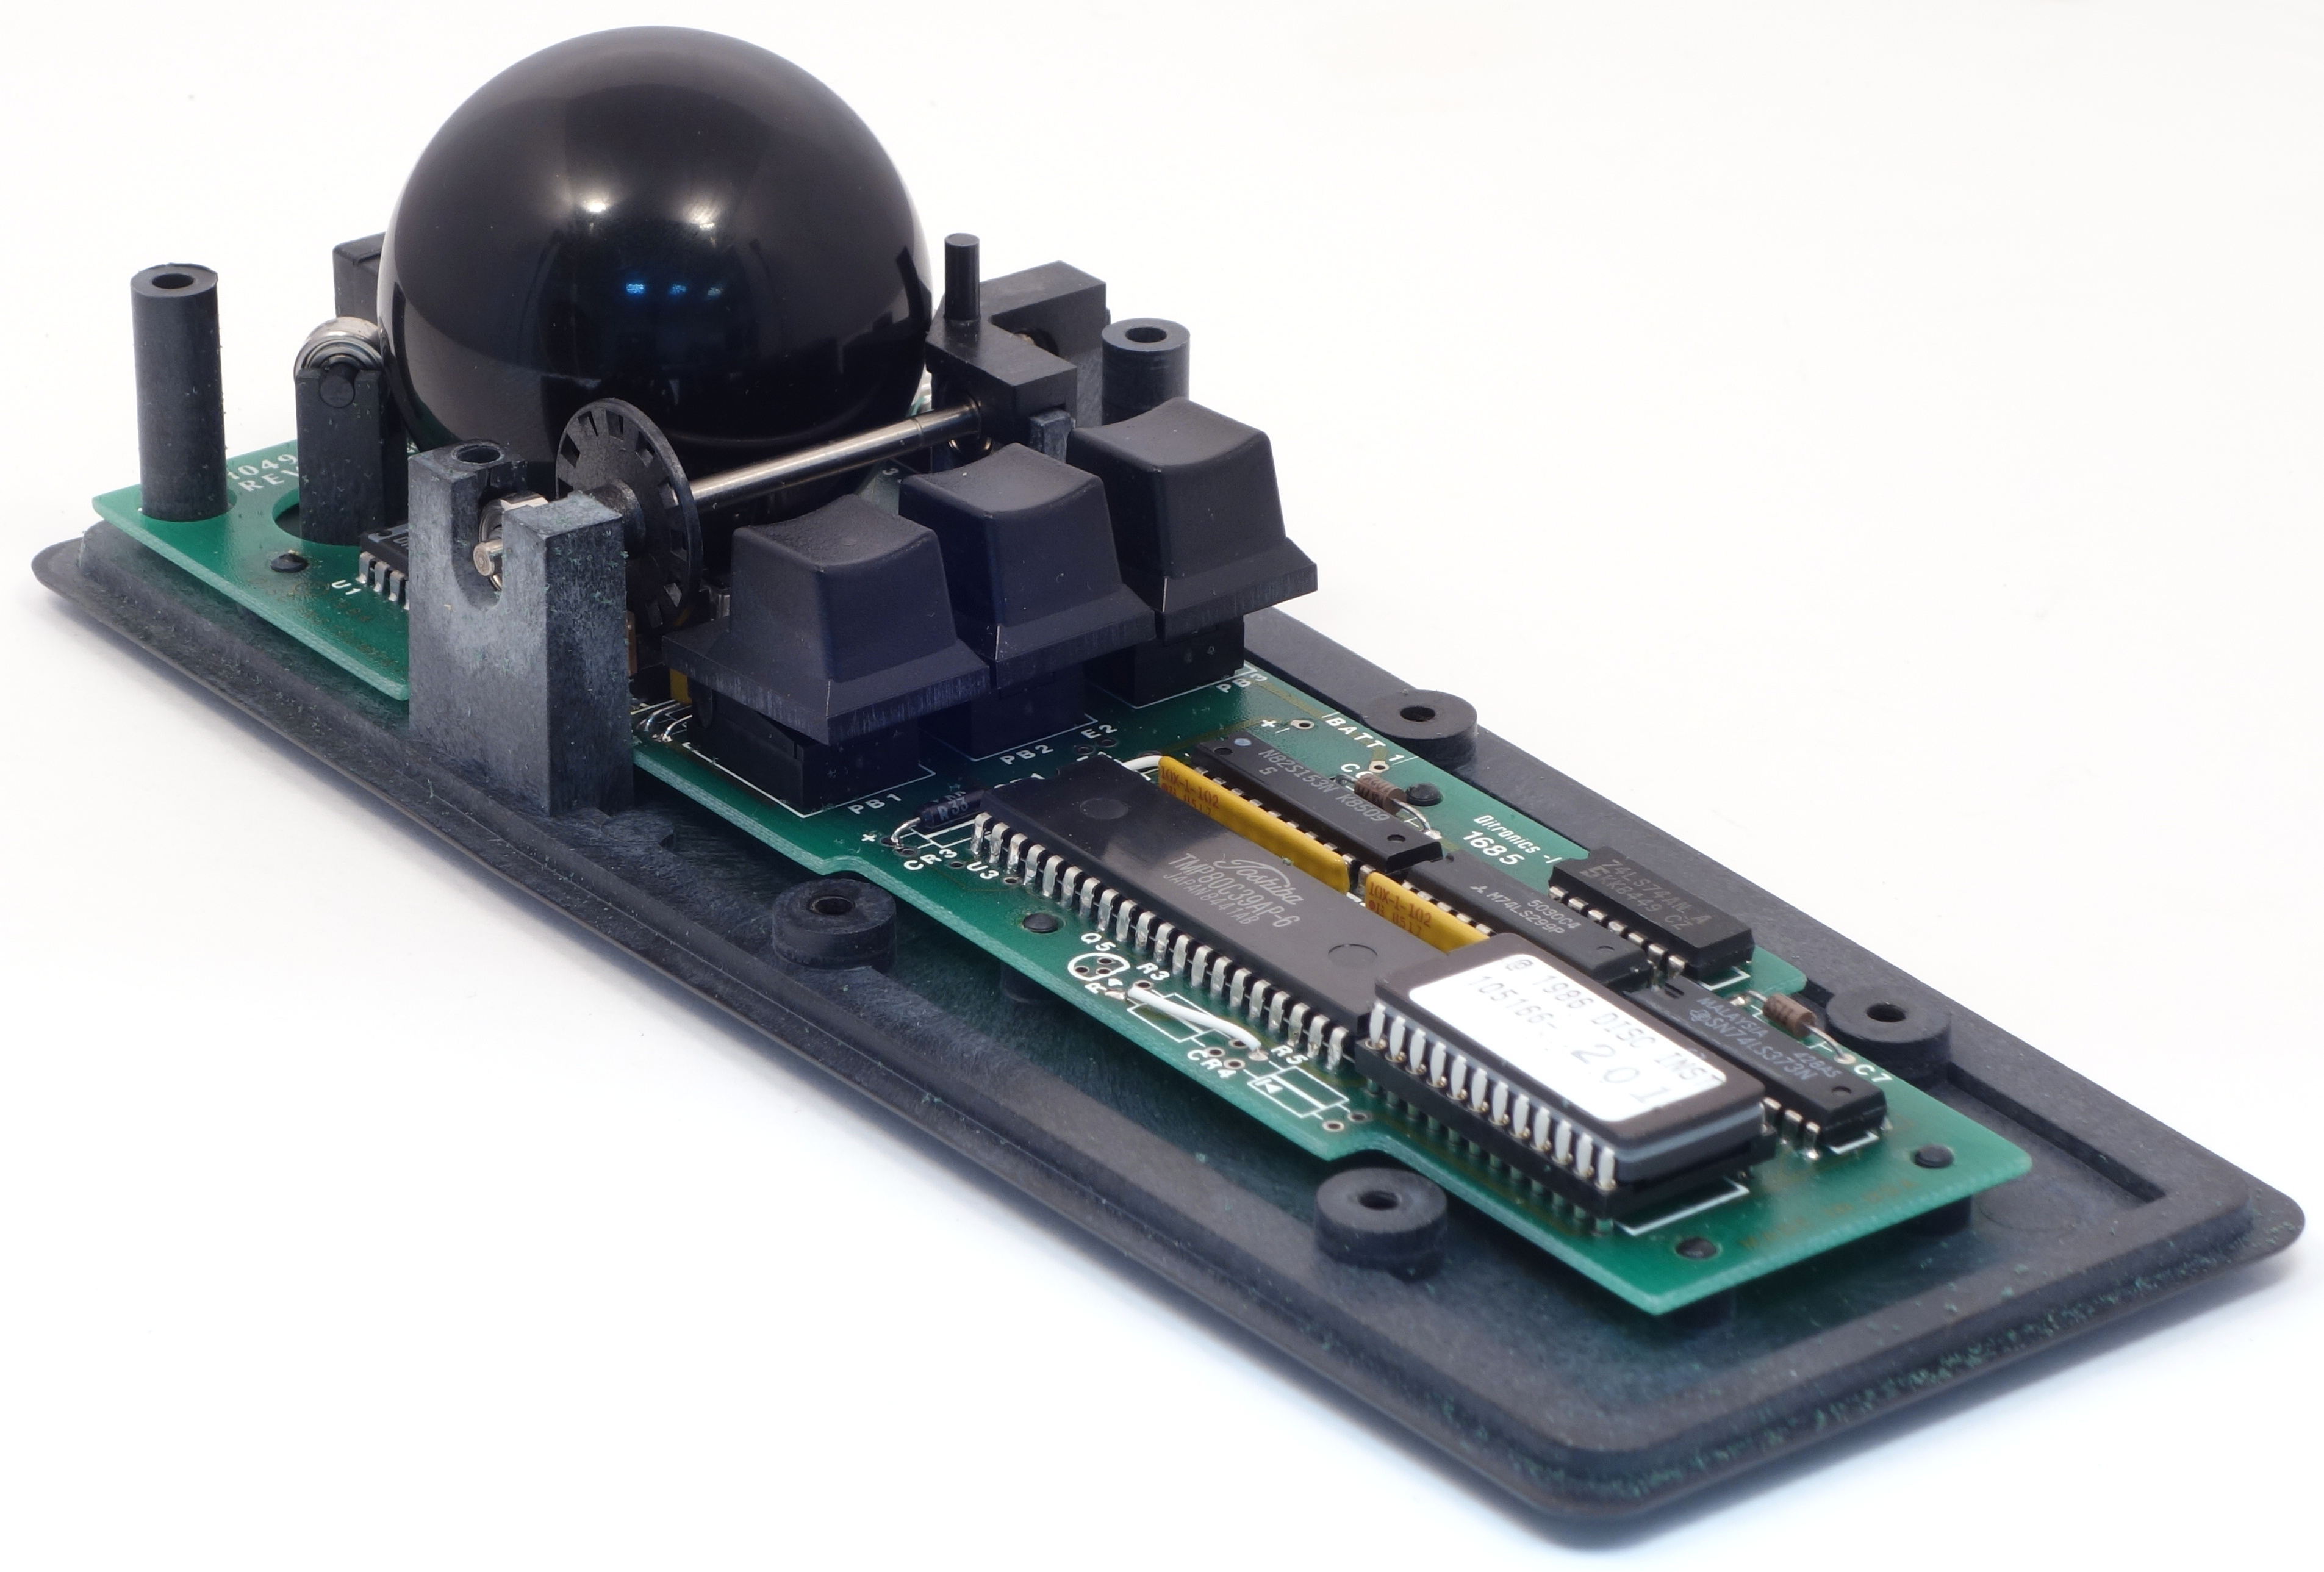
\includegraphics[scale=0.52]{1986_honeywell_microlynx_trackball/inside_60.jpg}
    \caption{microLYNX disassembled}
    \label{fig:microLYNXInside}
\end{figure}

Trackball internals are shown on figure \ref{fig:microLYNXInside}. This is an optomechanical device. Rollers are made using bearings and stainless steel shafts, which ensures maximum reliability and durability of the device. The high reliability of trackball and ergonomics, which is well suitable for a number of technical tasks, made this model “long-term survivor”: the device has been produced for at least ten years for industrial applications under various brands, and at the same time a constant appearance and mechanical part of the structure were preserved.

\begin{thebibliography}{9}
\bibitem {comlynx} Trackballs: Stationary mice // PC Magazine. August 1987, page 199-202 \url{https://trackballs.eu/media/Fulcrum/PC%20Mag%20Aug-1987%20p199-202.pdf}
\bibitem {lx200} Disc Instruments LX200 \url{https://web.archive.org/web/20220501213039/https://forum.trackballs.eu/viewtopic.php?f=17&t=16}
\end{thebibliography}
\end{document}
